\section{Resultados quantitativos}\label{sec:results}

\subsection{A curva de produtividade requerida}

O teto de 40 horas e o endpoint de 36 horas são objetos econômicos diferentes. Mover de 44 para 40 horas corta a cauda longa da distribuição formal usada como base e aproxima muitos trabalhadores do pico de eficiência assumido. Mover abaixo de 40 horas já não é sobretudo aparar fadiga; é retirar horas que o modelo trata como efetivas. Por isso a curva da Figura~\ref{fig:areq_curve} dobra para cima.

A Tabela~\ref{tab:mainresults} mostra os tetos de 40 e 36 horas, mas a comparação importante é a inclinação do caminho. A alternativa de 40 horas exige $1{,}53$--$1{,}57\%$ de PTF para restaurar o produto. O endpoint de 36 horas exige uma resposta maior: $6{,}52\%$ sob a hipótese de fadiga só acima de 40h e $8{,}38\%$ sob a penalidade bilateral. Essa diferença não é mero detalhe técnico. No primeiro caso, jornadas mais curtas não recebem penalidade direta de eficiência depois que as horas caem abaixo de 40. No segundo, afastar-se de 40 horas em qualquer direção tem custo de eficiência.

A margem formal--informal se move na direção esperada, mas não é a vilã do resultado agregado. A economia calibrada desloca alguns empregos marginais para a informalidade: em 36 horas, sua participação aumenta $2{,}28$ pontos percentuais sob fadiga só acima do pico e $2{,}92$ pontos sob penalidade bilateral. Ainda assim, a maior parcela negativa da variação do produto vem de menos horas físicas. Sem compensação de PTF, a perda líquida de produto é de $6{,}65\%$ e $8{,}40\%$, respectivamente. Em 40 horas, o produto cai $1{,}64\%$ e $1{,}68\%$.

% Generated by scripts/generate_assets.py; do not edit.
\begin{table}[!htbp]
\centering
\normalsize
\caption{Resultados nacionais da redução a partir de 44h, com ponte horária recalibrada}\label{tab:mainresults}
\setlength{\tabcolsep}{4pt}
\begin{tabular}{lrrrr}
\toprule
Indicador & \shortstack{Bilateral\\40h} & \shortstack{Bilateral\\36h} & \shortstack{Acima\\40h} & \shortstack{Acima\\36h} \\
\midrule
$\Delta Y$ (\%) & -1,677 & -8,398 & -1,636 & -6,646 \\
$A_{\mathrm{req}}$ (\%) & 1,573 & 8,381 & 1,534 & 6,524 \\
$A_{\mathrm{req}}$, composição fixa (\%) & 1,494 & 7,956 & 1,457 & 6,194 \\
Informalidade após reforma (\%) & 39,152 & 41,521 & 39,138 & 40,879 \\
$\Delta$ informalidade (p.p.) & 0,552 & 2,921 & 0,538 & 2,279 \\
$\Delta GHH$ (\%) & 0,225 & -4,366 & 0,276 & -2,121 \\
$CE$ (\% de $C_0$) & 0,176 & -3,420 & 0,216 & -1,661 \\
\bottomrule
\end{tabular}
\par\smallskip
\begin{minipage}{0.98\linewidth}\normalsize Fonte: PNAD Contínua 2024T4 reprocessada e simulações. Acima: fadiga somente acima do pico. Base: horas formais $\min\{h^{obs},44\}$, pesos PNAD preservados, horas informais inalteradas, informalidade de 38,600\%, $\sigma=1{,}326$; $\omega=0{,}675651$ (bilateral) e $0{,}676650$ (acima). A limitação inicial a 44h é uma hipótese de representação, não uma observação de horas contratuais. $A_{\mathrm{req}}$ recompõe o produto dessa base com composição reotimizada em cada avaliação; a variante fixa mantém a composição inicial. $\Delta Y$ usa $Y_0$, $\Delta GHH$ usa $GHH_0$ e $CE$ usa $C_0$ como denominador. Capital e ocupação totais fixos; cunhas são transferências e ajuste consome recursos.\end{minipage}
\end{table}


\begin{figure}[t]
\centering
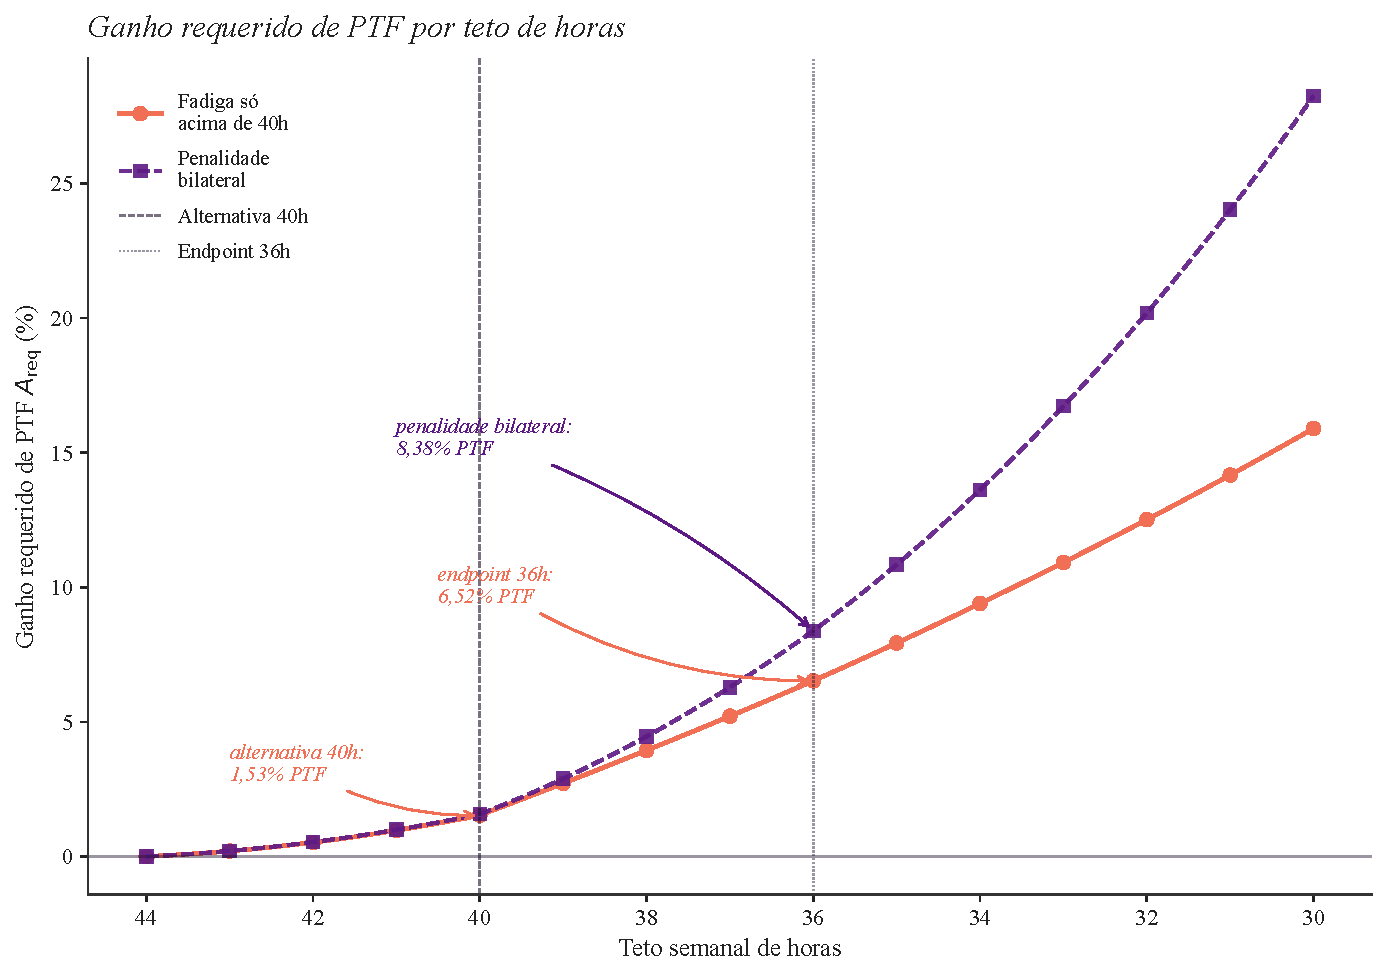
\includegraphics[width=0.92\textwidth]{generated/fig_areq_vs_hours_pt.pdf}
\caption{Ganho requerido de PTF $\Areq$ como função do teto semanal de horas.}\label{fig:areq_curve}
\tabnotes{A base limita previamente as horas habituais formais a 44h; esse teto é a referência sem reforma. A transformação aproxima a exposição ao limite legal, sem observar horas contratadas. $\Areq$ é assinado e restaura o produto com composição reotimizada. Os marcadores verticais distinguem 40h e 36h. Cada curva tem sua ponte horária e suas cunhas recalibradas. As funções $e(h)$ coincidem acima do pico, mas os agregados podem diferir pela eficiência inicial abaixo dele e pela calibração.}
\end{figure}

A figura também ajuda a ler o que o modelo está dizendo. As primeiras quatro horas de redução são baratas em unidades de PTF porque o canal de fadiga trabalha a favor da reforma. As quatro horas seguintes são caras porque a reforma passa a retirar trabalho efetivo. O apêndice mostra como esse diagnóstico depende das horas iniciais: preservar a cauda habitual acima de 44h reduz o requisito em 40 horas para cerca de $0{,}07\%$; em 36 horas, os valores passam a $5{,}00\%$ sob fadiga só acima do pico e $6{,}80\%$ sob penalidade bilateral. Por isso as magnitudes devem ser lidas como resultados da função calibrada de eficiência e da regra de base.
Sem nenhum canal de eficiência das horas, a base de 44h exige $2{,}40\%$ de PTF em 40 horas e $7{,}42\%$ em 36 horas, com ponte e cunhas recalibradas. A perda adicional de eficiência abaixo do pico explica por que, em 36h, a penalidade bilateral exige mais PTF que o cenário sem fadiga.

Congelar a composição formal--informal inicial reduz o requisito em 36 horas para $6{,}19\%$ sob fadiga só acima do pico e $7{,}96\%$ sob penalidade bilateral. A diferença decorre de a composição reotimizada responder ao objetivo privado com cunhas, e não somente ao produto. O apêndice apresenta essa comparação e as demais sensibilidades.

\subsection{Escala macroeconômica e mecanismos}

Ancoramos $\Areq$ no histórico brasileiro de PTF usando a série \texttt{rtfpna} da PWT 11.0 \citep{FeenstraInklaarTimmer2015,PWT2025,FREDPWTBrazil2026}. Essa comparação é uma régua de escala, não uma validação causal do contrafactual, pois o resíduo macro anual da PWT não é o mesmo objeto que a resposta de produtividade de curto prazo do modelo. A PTF brasileira caiu no período pós-1990, então um ganho único de seis e meio a oito e meio por cento é grande nessa régua. A alternativa de 40 horas está em outra região da escala. O apêndice traduz os ganhos únicos em taxas anualizadas para horizontes de três, cinco e dez anos; essa comparação de escala é mais informativa do que perguntar se uma década histórica específica ``repete'' o contrafactual.

\begin{figure}[t]
\centering
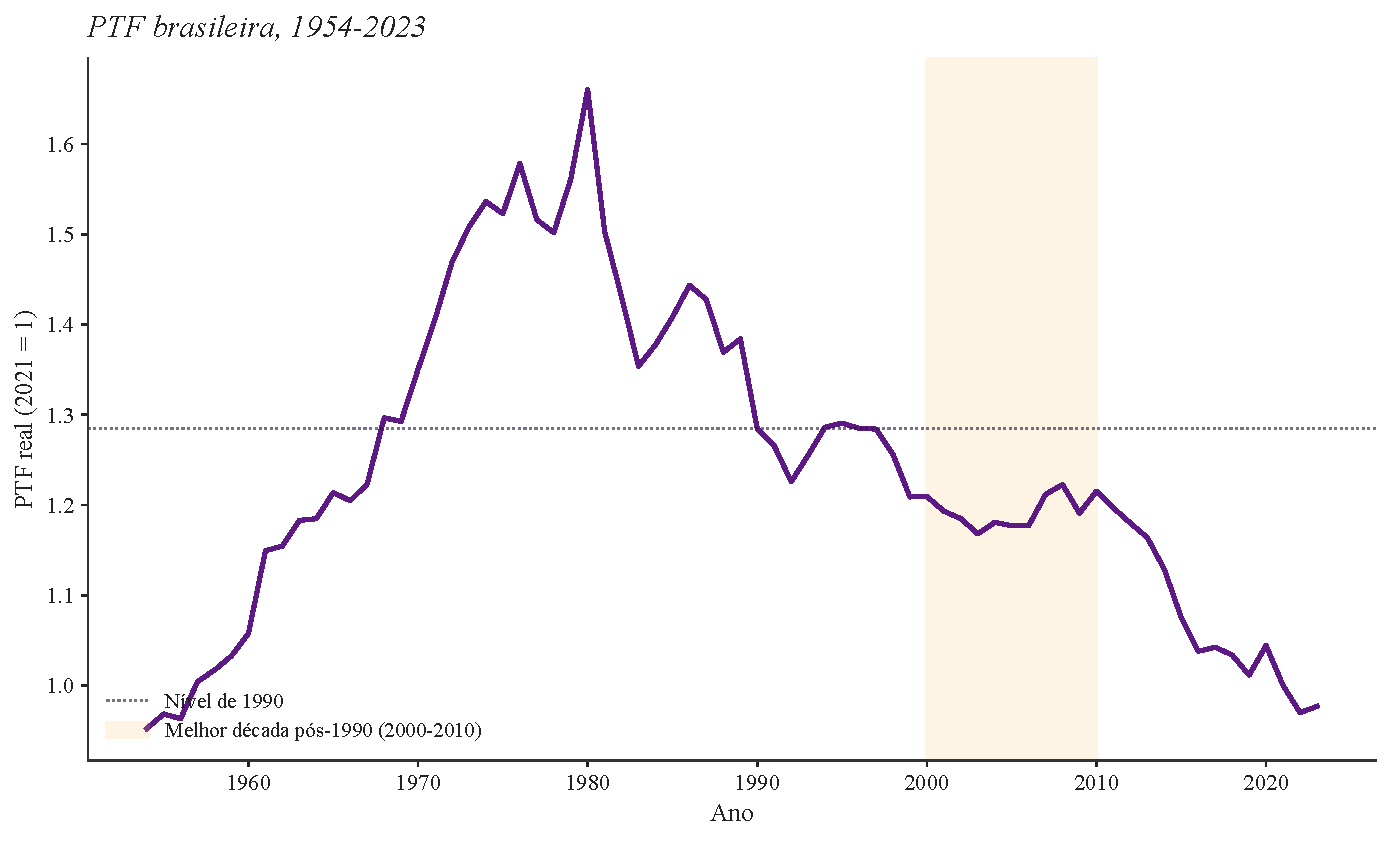
\includegraphics[width=0.95\textwidth]{generated/fig_areq_vs_tfp_history_pt.pdf}
\caption{PTF brasileira no longo prazo.}\label{fig:tfp_history}
\tabnotes{PTF real a preços nacionais constantes, série \texttt{rtfpna} da PWT 11.0, índice 2021 = 1. A linha horizontal marca o nível de 1990. A faixa destaca 2000--2010, a melhor janela de dez anos inteiramente contida em 1990--2019. Fonte: Penn World Table 11.0 via FRED, série \texttt{RTFPNABRA632NRUG}.}
\end{figure}

Para ilustrar a escala, repartir de forma composta o requisito de 36 horas por cinco anos corresponde a $1{,}27\%$ ao ano sob fadiga só acima do pico e $1{,}62\%$ sob penalidade bilateral. Na série brasileira, a queda anualizada foi de $0{,}83\%$ entre 1990 e 2023.

A decomposição esclarece o mecanismo. Na ordem horas físicas, eficiência e realocação, as parcelas em 36 horas sob penalidade bilateral são $-6{,}7070$, $-0{,}6622$ e $-1{,}0284$ pontos percentuais, totalizando $-8{,}3976\%$. Sob fadiga só acima do pico, a eficiência contribui positivamente, em $0{,}7066$ ponto, enquanto as horas físicas e a realocação contribuem com $-6{,}5397$ e $-0{,}8131$ pontos, totalizando $-6{,}6462\%$. Em 40 horas, sob penalidade bilateral, a perda física de $2{,}244$ pontos é parcialmente compensada pelo ganho de eficiência de $0{,}771$ ponto; a realocação adiciona perda de $0{,}204$ ponto. O apêndice reporta os níveis intermediários, sempre com o mesmo produto inicial como denominador.

\subsection{Bem-estar e heterogeneidade}\label{sec:welfare}

O cálculo de bem-estar deve ser lido como diagnóstico de consumo e lazer. Ele pergunta algo estreito: se emprego é fixo, salários não barganham e a reforma entrega mecanicamente mais tempo fora do trabalho aos incumbentes, o ganho de lazer compensa a perda de consumo? Isso não é um teorema de bem-estar social. Saúde, produção doméstica, barganha, preços, transições de emprego e pesos distributivos ficam fora do cálculo.

Dentro desse objeto estreito, a redução até 40 horas compra lazer a baixo custo de produto. O equivalente de consumo é de $+0{,}18\%$ sob penalidade bilateral e $+0{,}22\%$ sob fadiga só acima do pico; as variações do composto GHH são $+0{,}22\%$ e $+0{,}28\%$. Abaixo de 40 horas, o preço do lazer adicional sobe porque a reforma já não está apenas cortando fadiga de jornadas longas. Em 36 horas, o equivalente de consumo é de $-3{,}42\%$ sob penalidade bilateral e $-1{,}66\%$ sob fadiga só acima do pico; as variações GHH correspondentes são $-4{,}37\%$ e $-2{,}12\%$. As especificações concordam no sinal positivo da redução moderada e no sinal negativo do diagnóstico no endpoint.

\begin{figure}[t]
\centering
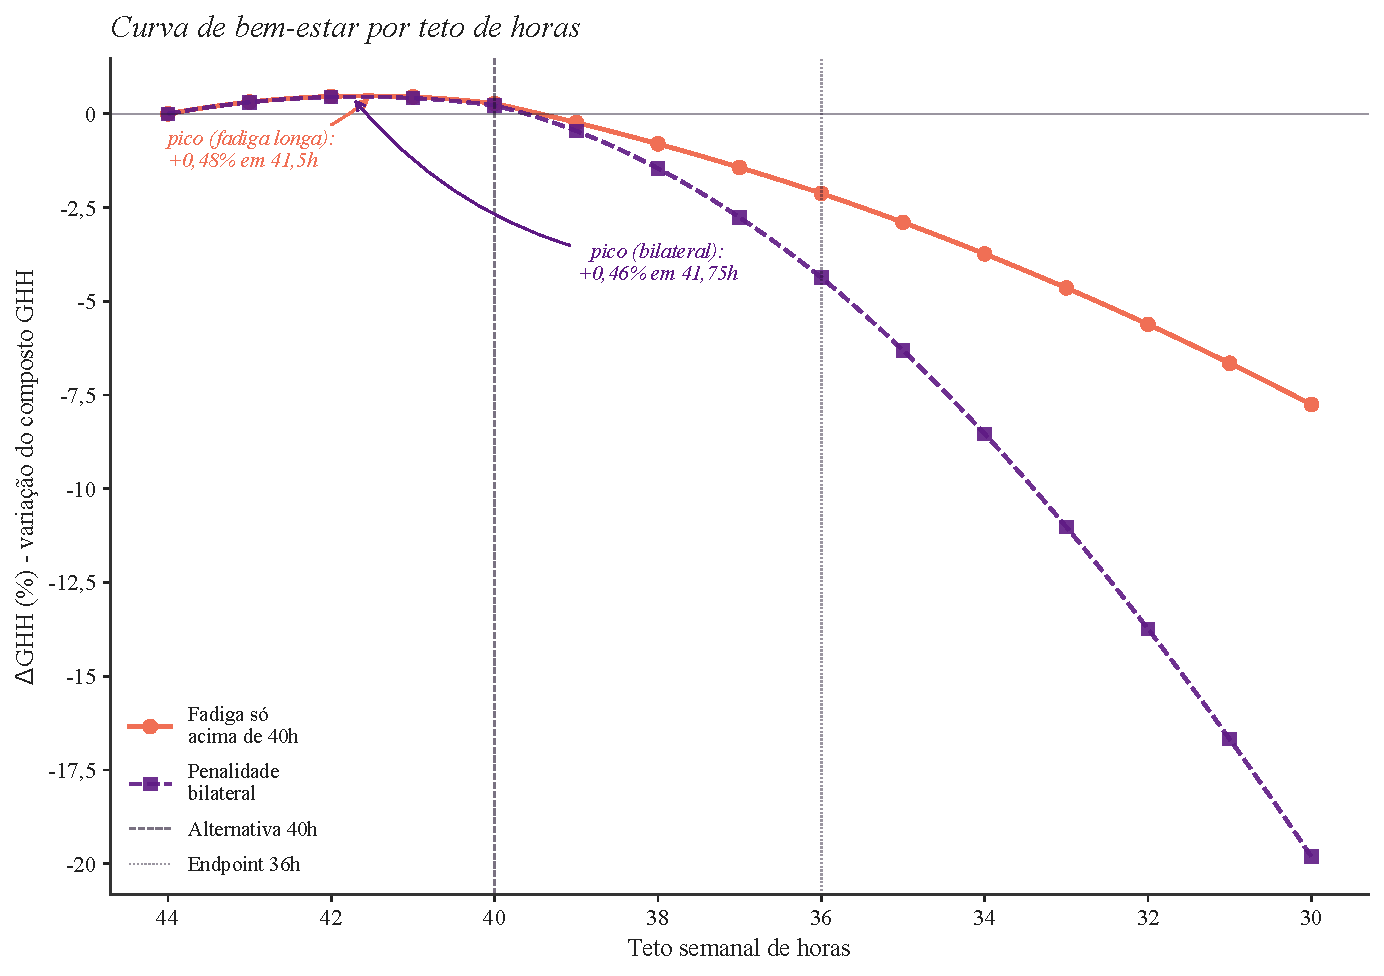
\includegraphics[width=0.92\textwidth]{generated/fig_welfare_schedule_pt.pdf}
\caption{Curva de bem-estar por teto de horas sob ambas as calibrações.}\label{fig:welfare_schedule}
\tabnotes{Variação percentual do composto GHH, com denominador $G_0$, conforme a Equação~\eqref{eq:cv}. Distribuição habitual formal limitada inicialmente a 44h, produtividade fixa e composição reotimizada. Os máximos anotados referem-se à grade de 0,25h sob preferências representativas; não identificam jornada socialmente ótima. O equivalente de consumo, com denominador $C_0$, é reportado separadamente na Tabela~\ref{tab:mainresults}.}
\end{figure}

Um ganho de PTF de aproximadamente $1{,}62\%$ no teto de 36h é suficiente para tornar o indicador GHH neutro sob fadiga só acima do pico. O limiar sob penalidade bilateral é de $3{,}40\%$. Ambos ficam abaixo do $\Areq$ neutro em produto porque o lazer compensa parcialmente a perda de consumo dentro desse objeto. O apêndice mostra esses limiares.

A curva do indicador GHH não implica oposição a reduções da jornada. Ela separa a perda de produto sob produtividade fixa, o ganho de produtividade que compensaria essa perda e o diagnóstico de consumo--lazer. Esses objetos não se movem juntos. O sinal do indicador depende da função de eficiência e da distribuição inicial: sem fadiga, o equivalente de consumo é negativo em 40 horas ($-0{,}67\%$) e em 36 horas ($-2{,}52\%$); na sensibilidade com horas habituais integrais, o equivalente de consumo em 36h passa a $-0{,}79\%$ no bilateral e $+0{,}96\%$ na fadiga só acima do pico. O agente representativo não permite decompor sua incidência entre trabalhadores.

Aplicar o arcabouço nacional separadamente a três setores amplos com momentos setoriais da PNAD entrega, no endpoint de 36 horas, um $\Areq$ de $8{,}85\%$ na agricultura, $8{,}97\%$ na indústria e $8{,}16\%$ nos serviços sob penalidade bilateral. Sob fadiga só acima do pico, os valores são $7{,}10\%$, $7{,}12\%$ e $6{,}31\%$. A informalidade sobe em todos os setores nesse teto. Para a alternativa de 40 horas, sob penalidade bilateral, os requisitos são $2{,}09\%$ na agricultura, $1{,}75\%$ na indústria e $1{,}50\%$ nos serviços. Esses são contrafactuais de equilíbrio parcial setor a setor, não uma análise de incidência insumo--produto. O apêndice online reporta os parâmetros, a decomposição completa e as sensibilidades.
